\documentclass{beamer}
% Green citations OR footnote citations. Biber???
% Two screens beamer
\usepackage{textpos} % package for the positioning
\usepackage{eso-pic}
\usepackage{tikz}
\usepackage{xstring}
\usepackage{xparse}

\usepackage[gen]{eurosym}

\newcommand{\dualscreen}{
\usepackage{pgfpages}
\setbeameroption{show notes on second screen}
\setbeamertemplate{note page}{\pagecolor{yellow!10}{\LARGE \insertnote}}
}

\newcommand{\noteline}{
{\\ \null \medskip}
}


\mode<presentation>
{
  \usetheme{Boadilla}
  \setbeamercovered{transparent}  % or whatever (possibly just delete it)
}

\usepackage{color}
\definecolor{arduteal}{RGB}{23, 161, 165}
\definecolor{uamai}{RGB}{26, 92, 153}   % Green shade for UAMAI, SjF, STU in Bratislava

\setbeamercolor{title}{fg=white,bg=uamai}% This is for the title (w/box)
\setbeamercolor{footnote mark}{fg=uamai} % Color of footnote marks (numbering) in beamer. Pretty darn hard to find.

% Overpic
\usepackage[percent]{overpic} % Writing over pics
 \usepackage[skins]{tcolorbox} % Nice color boxes

\newcommand{\tbox}[1]{\tcbox[enhanced,size=fbox,fontupper=\footnotesize,colback=white!100,drop fuzzy shadow southeast, sharp corners]{#1}}


\makeatletter
\newcommand{\slidefooter}[2]{
\setbeamertemplate{footline}
{
  \leavevmode%
  \hbox{%
  \begin{beamercolorbox}[wd=.333333\paperwidth,ht=2.25ex,dp=1ex,center]{section in head/foot}%
    \usebeamerfont{author in head/foot}\insertshortauthor~~\beamer@ifempty{\insertshortinstitute}{}{\insertshortinstitute}
  \end{beamercolorbox}%
  \begin{beamercolorbox}[wd=.333333\paperwidth,ht=2.25ex,dp=1ex,center]{section in head/foot}%
    \usebeamerfont{title in head/foot}\insertshorttitle
  \end{beamercolorbox}%
  \begin{beamercolorbox}[wd=.333333\paperwidth,ht=2.25ex,dp=1ex,right]{section in head/foot}%
    \usebeamerfont{date in head/foot}\insertshortdate{}\hspace*{2em}
    \insertframenumber{} / \inserttotalframenumber\hspace*{2ex}
  \end{beamercolorbox}}%

  \IfEqCase{#1}{
    {EN}{
      \IfEqCase{#2}{
        {STU}{
      \begin{tikzpicture}[remember picture,overlay]
            \node[anchor=south west,yshift=-0.7mm,xshift=-0.2mm] at (current page.south west) {
\includegraphics[height=2.5mm]{footer_EN_STU}};
      \end{tikzpicture}}
          {SjF}{
      \begin{tikzpicture}[remember picture,overlay]
            \node[anchor=south west,yshift=-0.5mm,xshift=-0.2mm] at (current page.south west) {
\includegraphics[height=2mm]{footer_EN_SjF}};
      \end{tikzpicture}}
      }
    }
    {SK}{
      \IfEqCase{#2}{
        {STU}{
      \begin{tikzpicture}[remember picture,overlay]
            \node[anchor=south west,yshift=-0.7mm,xshift=-0.2mm] at (current page.south west) {
\includegraphics[height=2.5mm]{footer_SK_STU}};
      \end{tikzpicture}}
          {SjF}{
      \begin{tikzpicture}[remember picture,overlay]
            \node[anchor=south west,yshift=-0.5mm,xshift=-0.2mm] at (current page.south west) {
\includegraphics[height=2.0mm]{footer_SK_SjF}};
      \end{tikzpicture}}
      }
    }
  }

  \vskip0pt%
}
}
\makeatother



\setbeamercolor{toptitlecolor}{fg=white,bg=uamai}
\makeatletter
\setbeamertemplate{frametitle}
{\vskip-3pt
  \leavevmode
  \hbox{%
  \begin{beamercolorbox}[wd=\paperwidth,ht=2.7ex,dp=1.2ex]{toptitlecolor}%
    \raggedright\hspace*{0.4em}\large\insertframetitle
  \end{beamercolorbox}
  }%
}
\makeatother

\setbeamercolor{very important text}{fg=white,bg=uamai}
\newcommand{\veryimportant}[1]{{%
  \usebeamercolor{very important text}\colorbox{bg}{\textcolor{black}{#1}}%
}}

\newcommand{\important}[1]{\ignorespaces\textcolor{uamai}{#1}}

\setbeamercolor{alerted text}{fg=uamai}

\newcommand{\slideheader}[1]{

  \IfEqCase{#1}{
    {EN}{
    \addtobeamertemplate{frametitle}{}{%
    \begin{tikzpicture}[remember picture,overlay]
        \node[anchor=north east,yshift=7.9mm,xshift=4.5mm] at (current page.north east) {\includegraphics[height=2cm]{uamai}};
    \end{tikzpicture}}
    }
    {SK}{
    \addtobeamertemplate{frametitle}{}{%
    \begin{tikzpicture}[remember picture,overlay]
        \node[anchor=north east,yshift=-0mm,xshift=0mm] at (current page.north east) {
\includegraphics[height=5mm]{urkLogoWhite}};
    \end{tikzpicture}}
    }
  }
}

\makeatletter
\definecolor{beamer@blendedblue}{RGB}{26, 92, 153}
\makeatother

\definecolor{UAMAIgreen}{RGB}{26, 92, 153}

 \usepackage{graphicx}
\graphicspath{{./figs/}}
\usepackage{epstopdf} %Converts EPS to PDF so PDFLaTeX can be used
\newcommand{\figone}[0] {1.000\textwidth} %Multiplier for all single full width images
\newcommand{\figtwo}[0] {0.48\textwidth} %Multiplier for all double half width images
\newcommand{\figthree}[0] {0.321\textwidth} %Multiplier for all triple third width images
\newcommand{\figtwoh}[0] {0.3\textheight} %Multiplier for all double half width


\usepackage{subfigure}
\usepackage{amsfonts}
\usepackage{amssymb}
\usepackage{amsmath}
\usepackage{theorem}
\usepackage{epsfig}
\usepackage{mathrsfs} %mathscr
\usepackage[utf8]{inputenc}
\usepackage[T1]{fontenc}
\usepackage{courier} % To get courier fonts in listings
\usepackage{listings}
\lstset{basicstyle=\normalsize\ttfamily,breaklines=true,numbers=left,xleftmargin=2em,frame=single,framexleftmargin=1.5em}

\lstdefinelanguage{Arduino}[]{C++}      %Defining Arduino
{morekeywords={setup,loop,function,pgm_read_float,pgm_read_word,PROGMEM,pinMode,digitalWrite,digitalRead,analogReference,analogRead,analogWrite,analogReadResolution,analogWriteResolution,tone,noTone,shiftOut,shiftIn,pulseIn,millis,micros,delay,delayMicroseconds,min,max,abs,constrain,map,pow,sqrt,sin,cos,tan,isAlphaNumeric,isAlpha,isAscii,isWhitespace,isControl,isDigit,isGraph,isLowerCase,isPrintable,isPunct,isSpace,isUpperCase,iisHexadecimalDigit,randomSeed,random,lowByte,highByte,bitRead,bitWrite,
bitSet,bitClear,bit,attachInterrupt,detachInterrupt,interrupts,noInterrupts,Serial,Stream,Keyboard,Mouse},
sensitive=true,
alsoletter={_}
}

\lstdefinelanguage{myArduino}[]{Arduino}      %Defining my own Arduino
{morekeywords={OptoShield,HeatShield,begin,calibration,sensorRead,actuatorWrite,referenceRead,compute,PIDAbs,step},
sensitive=true,
alsoletter={_},
numbers=left,
xleftmargin=2em,
xrightmargin=0.2em,
frame=single,
framexleftmargin=1.5em
}

%Extended Matlab language
\lstdefinelanguage{myMatlab}[]{Matlab}      {morekeywords={ectrl.exportToC,cost,LTISystem,QuadFunction,MPCController,toExplicit,partition,feedback,fplot,function,arduino,writeDigitalPin,textscan,fminsearch,dlqr,predmodelqp,dlyap,ones,linprog,quadprog,optimset,qpOASES,qpOASES_sequence,sysStruct,probStruct,mpt_control,volume,hull,extreme,mpt_exportc,mpt_getInput,sdpvar,blkdiag,sdpsettings,solvesdp,geomean,double,},
sensitive=true,
alsoletter={_}
numbers=left,
xleftmargin=2em,
frame=single,
framexleftmargin=1.5em
}

\lstdefinelanguage{myPython}[]{Python}
{morekeywords={},
sensitive=true,
alsoletter={_}
numbers=left,
xleftmargin=2em,
frame=single,
framexleftmargin=1.5em}

\lstdefinelanguage{myBash}[]{bash}
{morekeywords={},
sensitive=true,
alsoletter={_}
numbers=left,
xleftmargin=2em,
frame=single,
framexleftmargin=1.5em}

\lstdefinestyle{customc}{
  belowcaptionskip=1\baselineskip,
  breaklines=true,
  xleftmargin=\parindent,
  language=myArduino,
  showstringspaces=false,
  basicstyle=\normalsize\ttfamily,
  keywordstyle=\bfseries\color{green!40!black},
  commentstyle=\itshape\color{purple!40!black},
  identifierstyle=\color{blue},
  stringstyle=\color{orange},
}

\lstdefinestyle{custompython}{
  belowcaptionskip=1\baselineskip,
  breaklines=true,
  xleftmargin=\parindent,
  language=myPython,
  showstringspaces=false,
  basicstyle=\normalsize\ttfamily,
  keywordstyle=\bfseries\color{green!40!black},
  commentstyle=\itshape\color{purple!40!black},
  identifierstyle=\color{blue},
  stringstyle=\color{orange},
}

\lstdefinestyle{custommatlab}{
  belowcaptionskip=1\baselineskip,
  breaklines=true,
  xleftmargin=\parindent,
  language=myMatlab,
  showstringspaces=false,
  basicstyle=\normalsize\ttfamily,
  keywordstyle=\bfseries\color{green!40!black},
  commentstyle=\itshape\color{purple!40!black},
  identifierstyle=\color{blue},
  stringstyle=\color{orange},
 }


\lstnewenvironment{arduino}[1]{
\lstset{
language=myArduino,
caption=#1,
label=#1,
style=customc}
}
{
}

%Plain with no numbering
\lstnewenvironment{ardu}{
\lstset{
language=myArduino,
style=customc}
}
{
}

\lstnewenvironment{matlab}[1]{
\lstset{
language=myMatlab,
caption=#1,
label=#1,
style=custommatlab}
}
{
}

\lstnewenvironment{mtlb}{
\lstset{
language=myMatlab,
style=custommatlab}
}
{
}

%----------------------------------------------------
\newcommand{\muaompc}{$\mu${AO-MPC}}

\renewcommand{\vec}[1]{\boldsymbol{\mathrm{#1}}} %Bold vectors instead of arrows

%This custom command defines how the literal menus look like.
\newcommand{\gui}[1]{{\emph{#1}}} %Gui commands, icon names, buttons

% All code, functions, variables are typed like this
\newcommand{\code}[1]{{\lstinline[columns=fixed]{#1}}} %Shorthand for code


\usepackage[framed,numbered,autolinebreaks,useliterate]{mcode}



% REFERENCE RELATED COMMANDS
% ----------------------------------------------------
% Generic reference related

\newcommand{\citep}[1]{
{\color{uamai} [\cite{#1}]}
}

%\setbeamercolor{bibliography item}{parent=red}
\setbeamercolor*{bibliography entry title}{fg=black}
\setbeamercolor*{bibliography entry author}{fg=uamai}
\setbeamercolor*{bibliography entry journal}{fg=uamai}
\setbeamercolor*{bibliography entry note}{fg=black}
% -----------------------------------------------------
% References specific for BiBTeX
% -----------------------------------------------------
\newcommand{\referencesslide}[2]{
\referencebegin

  \IfEqCase{#2}{
    {EN}{
    \begin{frame}[allowframebreaks,plain]{References}
    }
    {SK}{
    \begin{frame}[allowframebreaks,plain]{Bibliografia}
    }
  }
    \small
    \bibliographystyle{apalike}
    \bibliography{#1}
    \end{frame}
\referenceend
}

\newcommand{\bibliographyfile}[2]{
    \IfEqCase{#2}{
    {EN}{
            \usepackage[
            citestyle       = authoryear,
            doi             = false,
            isbn            = false,
            url             = false,
            maxcitenames    = 1,
            backend         = biber
            ]{biblatex}
            \addbibresource{#1}
            \AtBeginBibliography{\small}
            \AtEveryCitekey{\iffootnote{\color{uamai}\scriptsize}{\color{uamai}}}
        }
    {SK}{
            \usepackage[slovak]{babel}
            \usepackage[
            citestyle       = authoryear,
            doi             = false,
            isbn            = false,
            url             = false,
            maxcitenames    = 1,
            backend         = biber
            ]{biblatex}
            \DefineBibliographyStrings{slovak}{
            andothers = {{a\ kol\adddot}},
            }
            \addbibresource{#1}
            \AtBeginBibliography{\small}
            \AtEveryCitekey{\iffootnote{\color{uamai}\scriptsize}{\color{uamai}}}
        }
     }
}

% References slide for biber
\newcommand{\referencesslidebiber}[1]{
\referencebegin

  \IfEqCase{#1}{
    {EN}{
    \begin{frame}[allowframebreaks,plain]{References}
    }
    {SK}{
    \begin{frame}[allowframebreaks,plain]{Bibliografia}
    }
  }
    \printbibliography
    \end{frame}
\referenceend
}

% END REFERENCE RELATED COMMANDS
% -----------------------------------------------------

%%% Formatting captions
\usepackage{caption}
\DeclareCaptionFont{tiny}{\tiny}
\captionsetup{font=scriptsize} % Font size
\captionsetup{labelformat=empty} % No labels
\captionsetup{justification=centering} % Centered

%%% Title font
\setbeamerfont{title}{size=\Large,parent=structure} % Bold fonts

%%% Remove navigation
\setbeamertemplate{navigation symbols}{} % No navigation buttons, they are useless

% Rectangles for decoration
\usepackage{tikz}
\usetikzlibrary{shapes}

% Author email address command
\newcommand{\email}[1]{\url{#1}}





\newcommand{\referencebegin}{
   \newcounter{framenumberappendix}
   \setcounter{framenumberappendix}{\value{framenumber}}
}

\newcommand{\referenceend}{
   \addtocounter{framenumberappendix}{-\value{framenumber}}
   \addtocounter{framenumber}{\value{framenumberappendix}}
}


\newcommand{\reviewbegin}{
   \newcounter{framenumberreview}
   \setcounter{framenumberreview}{\value{framenumber}}
}

\newcommand{\reviewend}{
   \addtocounter{framenumberreview}{-\value{framenumber}}
   \addtocounter{framenumber}{\value{framenumberreview}}
}

\newcommand{\backupbegin}{
   \newcounter{framenumberreview}
   \setcounter{framenumberreview}{\value{framenumber}}
}

\newcommand{\backupend}{
   \addtocounter{framenumberreview}{-\value{framenumber}}
   \addtocounter{framenumber}{\value{framenumberreview}}
}


% Thank you slide
\newcommand{\thankyouslide}[2]{
\begin{frame}[plain]

\begin{tikzpicture}[remember picture, overlay]

\fill[UAMAIgreen] (-1,-2.8) rectangle (10.2,-4.2);
\end{tikzpicture}

  \IfEqCase{#2}{
    {EN}{
    \vspace{8em}
      {\Huge Thank you for your attention!}
      \vspace{9em}\\
      Please feel free to contact me any time at
     \url{#1}
    }
    {SK}{
    \vspace{8em}
      \color{white}{\Huge Ďakujem za Vašu pozornosť.}
      \vspace{9em}\\
      Môžete ma kontaktovať hocikedy na adrese
     \url{#1}
    }
    {AS}{
\begin{tikzpicture}[remember picture, overlay]
 \node[anchor=north west] (aslogo) at ([xshift=1.3cm,yshift=-0.3cm]current page.north west)
       {\includegraphics[width=10cm]{automationshield}};
\fill[UAMAIgreen] (-2,-3.0) rectangle (10.2,-4.2);
\end{tikzpicture}

\vspace{7.5em}
{\Huge Thank you for your attention!}
\vspace{4em}\\
Make sure to visit \url{www.automationshield.com} for more information.
\vfill
Please feel free to contact me any time at
\url{#1}

    }
  }
\addtocounter{framenumber}{-1}
\end{frame}
}

\newcommand{\titleslide}[3][]{

    \lstset{aboveskip=3pt, belowskip=3pt} %Space above and below lstlist boxes
    \begin{frame}[plain]

    \begin{tikzpicture}[remember picture, overlay]
    \node (logo background) [shape=rectangle, fill=white, minimum height=1.3cm, minimum width=80mm, anchor=south west] at ([xshift=7.5cm,yshift=1.5cm]current page.south west) {};
    \end{tikzpicture}

    %detect if optional argument

  \IfEqCase{#2}{
    {EN}{
    \begin{tikzpicture}[remember picture, overlay]
        \node[anchor=south west] (uamai) at ([xshift=7cm,yshift=0.5cm]current page.south west)
        {\includegraphics[height=3cm]{uamai}};
    \end{tikzpicture}
    }
    {SK}{
    \begin{tikzpicture}[remember picture, overlay]
        \node[anchor=south west] (urkLogo) at ([xshift=8.3cm,yshift=1.5cm]current page.south west)
        {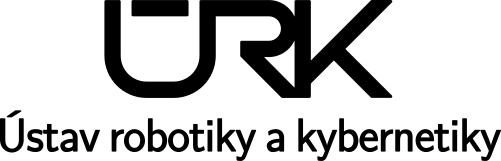
\includegraphics[height=10mm]{urkLogo}};
    \end{tikzpicture}
    }
  }

  \IfEqCase{#3}{
    {STU}{
    \begin{tikzpicture}[remember picture, overlay]
        \node[anchor=south west] (stu) at ([xshift=0.5cm,yshift=0.5cm]current page.south west)
        {\includegraphics[height=3cm]{stu}};
    \end{tikzpicture}
    }
    {STU_EXT}{
    \begin{tikzpicture}[remember picture, overlay]
        \node[anchor=south west] (stuext) at ([xshift=-0.5cm,yshift=0.9cm]current page.south west)
        {\includegraphics[height=2.2cm]{stuext}};
    \end{tikzpicture}
    }
    {SjF}{
    \begin{tikzpicture}[remember picture, overlay]
        \node[anchor=south west] (sjf) at ([xshift=0.5cm,yshift=0.5cm]current page.south west)
        {\includegraphics[height=3cm]{sjf}};
    \end{tikzpicture}
    }
    {SjF_EXT}{
    \begin{tikzpicture}[remember picture, overlay]
        \node[anchor=south west] (sjfext) at ([xshift=-0.5cm,yshift=0.9cm]current page.south west)
        {\includegraphics[height=2.2cm]{sjfext}};
    \end{tikzpicture}
    }
  }

  \titlepage

\vspace{1.3cm}

\setbox0=\hbox{#1\unskip}\ifdim\wd0=0pt

  %\hfill\insertshortdate{}

\else
    \IfEqCase{#2}{
    {EN}{
    Thesis supervisor: #1 \hfill \insertshortdate{}
     }
    {SK}{
    Vedúci práce: #1 \hfill \insertshortdate{}
     }

    }
\fi




  \addtocounter{framenumber}{-1}

\end{frame}
}

\newenvironment{reviewerquestions}[1]
{
\reviewbegin                                 % Use this to answer reviewer / Používať na predpripravené odpovede na oponentské otázky
  \IfEqCase{#1}{
    {EN}{
    \begin{frame}[allowframebreaks,plain]{Reviewer's questions} % {Otázky oponenta}
    }
    {SK}{
      \begin{frame}[allowframebreaks,plain]{Otázky oponenta} % {Otázky oponenta}
    }
  }
}
{
\end{frame}
\reviewend                                  % Use this to answer reviewer / Používať na pripravené odpovede na oponentské otázky
}
 %bugfix
\makeatletter
\let\@@magyar@captionfix\relax
\makeatother



\usepackage{xspace} % Backspace. Prevents certain commands to eating spaces.
\newcommand{\Ohm}{$\Omega$\xspace} % Ohms
\newcommand{\E}[1]{$\mathrm{E}{#1}$} % Engineering notation

%\dualscreen

\newcommand{\angl}[1]{{\color{gray}(\emph{angl.:} #1)}}


\title[Riadiace Algoritmy Dronov]
{Working title drone control}
\subtitle{\vspace{1em}Riadenie dronov}
\author[]{prof. Ing. Gergely Takács, PhD.}
\date[07.12.2021]{}
\slideheader{SK}
\slidefooter{SK}{STU}
\bibliographyfile{gergelytakacsBibliography.bib}{SK}


\begin{document}
\titleslide[]{SK}{STU}


%viem si predstavit klasika kaskadne riadenie ala arducopter
%%potom mozno LQR a Integral backstepping a vysvetlit co ma aku vyhodu ...

%%\begin{frame}[fragile]{Test tikz}
%
%
%    \begin{figure}[ht]
%        \begin{center}
%            \begin{tikzpicture}[auto, node distance=1cm,>=latex']
%            \node [input, name=input] {};
%            \node [sum, right=of input] (sum) {};
%            \node [block, right=of sum] (controller) {$C(s)$};
%            \node [block, right=2 of controller] (plant) {$G(s)$};
%            \node [output, right=of plant] (output) {};
%
%            \draw [draw,->] (input) -- node {$U(s)$} (sum);
%            \draw [->] (sum) -- node {} (controller);
%            \draw [->] (controller) -- node {} (plant);
%            \draw [->] (plant) -- node [name=y] {$Y(s)$}(output);
%            \draw [->] (y) -- ++ (0,-2) -| node [pos=0.99] {$-$} (sum);
%            \end{tikzpicture}
%        \end{center}
%    \end{figure}

%\end{frame}

%
\begin{frame}[t]{Motivácia: Počítače sú všade okolo nás...}
\begin{columns}
\begin{column}{.48\textwidth}
\begin{onlyenv}<1-2>
Text \cite{Cholodwicz2017}
\begin{figure}
\centering
  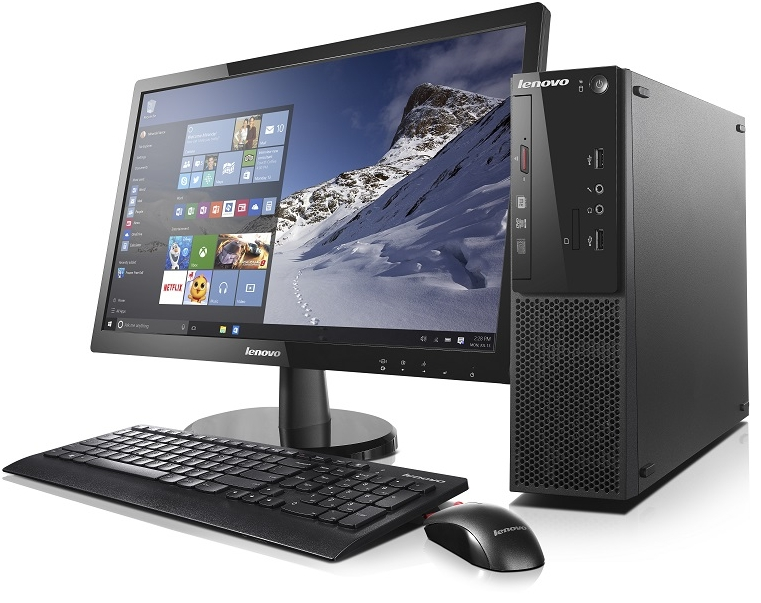
\includegraphics[height=55mm]{pc}\\
\end{figure}
\end{onlyenv}
\end{column}
\begin{column}{.48\textwidth}
\begin{onlyenv}<2>
\begin{figure}
\centering
  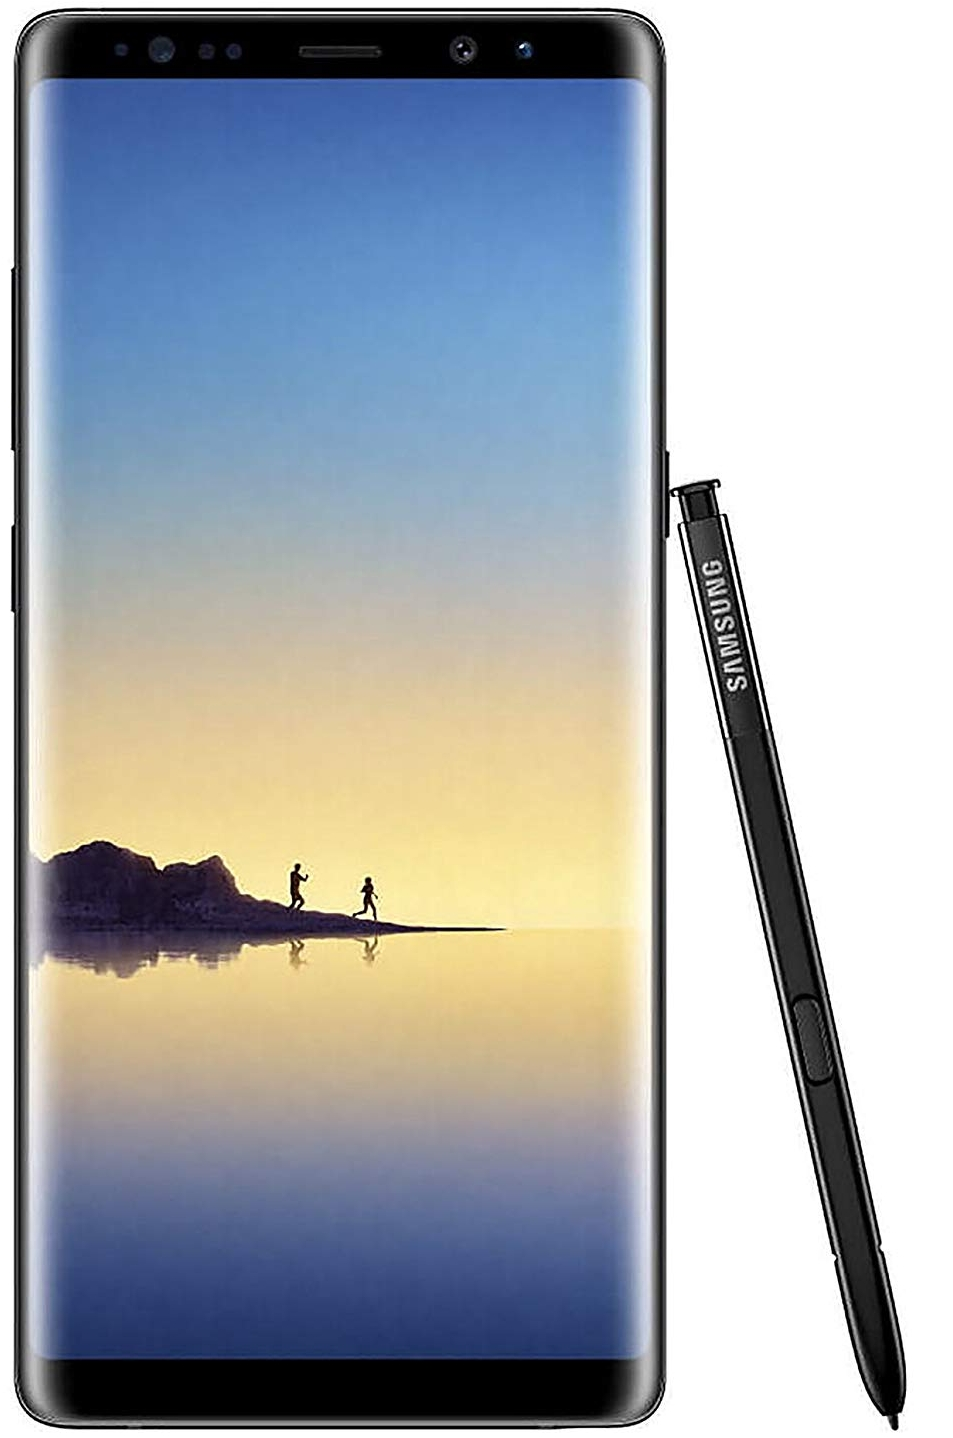
\includegraphics[height=55mm]{phone}\\
\end{figure}
\end{onlyenv}
\end{column}
\end{columns}
\end{frame}



\begin{frame}{Opakovanie: Riadená sústava}
  \begin{itemize}
    \item<1-> Riadená sústava, systém alebo proces \angl{plant, system, process}, v tomto prípade celá kvadrikoptéra
    \item<2-> Vstup $u(t)$ \angl{input} sú akčné zásahy, napr. PWM/RC do motorov
    \item<3-> Výstup $y(t)$ \angl{output} je meraná, tzv. manipulovaná veličina \angl{manipulated variable}; napr. klopenie $\theta(t)$ drona
    \item<4-> Porucha \angl{disturbance} $w(t)$ je vplyv vonkajšieho prostredia, napr. vietor
  \end{itemize}

\begin{figure}
\centering
  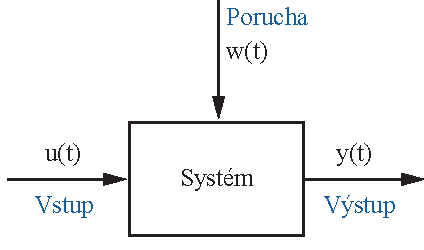
\includegraphics[width=60mm]{loop_1}\\
\end{figure}
\end{frame}

\begin{frame}{Opakovanie: Meranie}
  \begin{itemize}
    \item<1-> Výstupy $y(t)$ sú idealizované
    \item<2-> Poruchy, teda šum merania $v(t)$ a dynamika snímača vplýva na výsledok
    \item<3-> Merania môžeme korigovať, resp. nemerané veličiny odhadnúť $\hat{y}(t)$
    \item<4-> Pre jednoduchosť často predpokladáme ideálne meranie ${y}(t)=\hat{y}(t)$
  \end{itemize}

\begin{onlyenv}<1-3>
\begin{figure}
\centering
  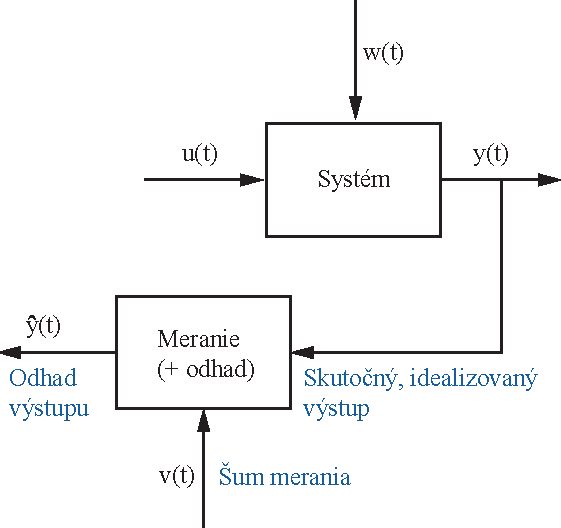
\includegraphics[width=60mm]{loop_2}\\
\end{figure}
\end{onlyenv}


\begin{onlyenv}<4>
\begin{figure}
\centering
  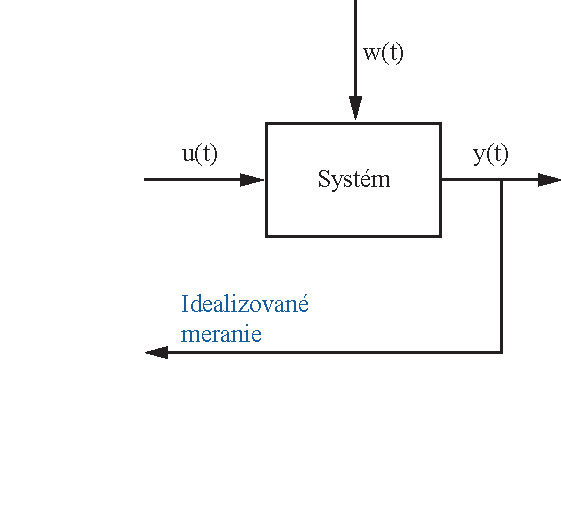
\includegraphics[width=60mm]{loop_2b}\\
\end{figure}
\end{onlyenv}
\end{frame}

\begin{frame}{Opakovanie: Riadiacia odchýlka}
  \begin{itemize}
    \item<1-> Žiadaná hodnota alebo referencia \angl{setpoint, reference} $r(t)$ vyjadruje na akú hodnotu chceme dostať výstup, potom
    \item<2-> Rozdiel medzi žiadanou hodnotou a výstupom $e(t)=r(t)-y(t)$ je odchýlka riadenia \angl{error}
  \end{itemize}

\begin{figure}
\centering
  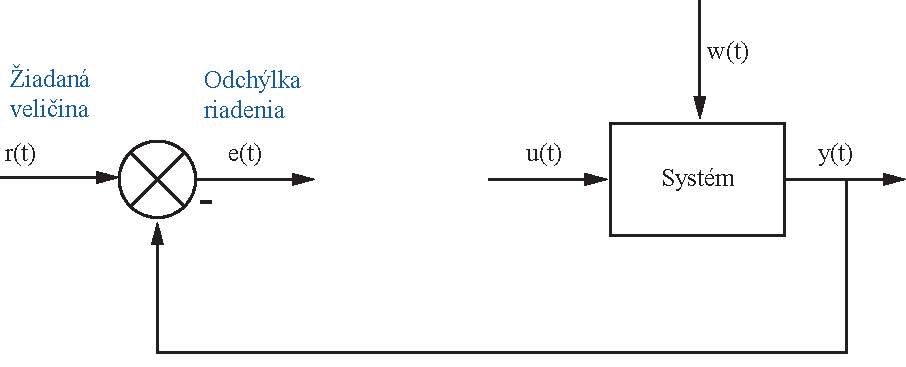
\includegraphics[width=100mm]{loop_ref}\\
\end{figure}
\end{frame}


\begin{frame}[t]{Opakovanie: Riadiaci algoritmus}
  \begin{itemize}
    \item<1-> Riadenie je logika ktorá prepočíta odchýlku riadenia $e(t)$ na vstupy $u(t)$
    \item<2-> Môže to byť ľubovoľné, do konca aj analógové a mechanické (e.g. riadenie rýchlosti parného stroja)
    \item<3-> Dobrým kompromisom medzi komplexnosťou (pochopenie, návrh) a implementovateľnosťou je PID riadenie
    \item<4-> Až 97\% riadiacich algoritmov v praxi sú PID... \citep{Murray2004}
    \item<5-> ...a väčšina z nich sú slabo naladené\footnote{ArduPilot: ``most heli users have not learned how to tune up their helis yet'' \citep{Hall2020}}
  \end{itemize}

\begin{onlyenv}<1>
\begin{figure}
\centering
  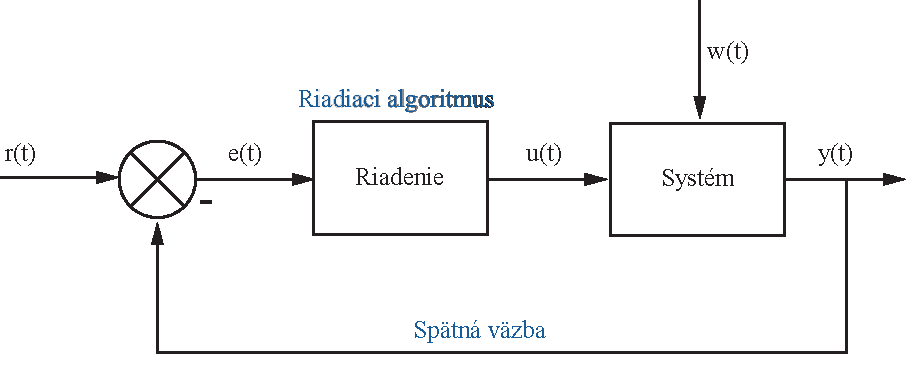
\includegraphics[width=80mm]{loop_all}\\
\end{figure}
\end{onlyenv}

\begin{onlyenv}<2>
\begin{figure}
\centering
  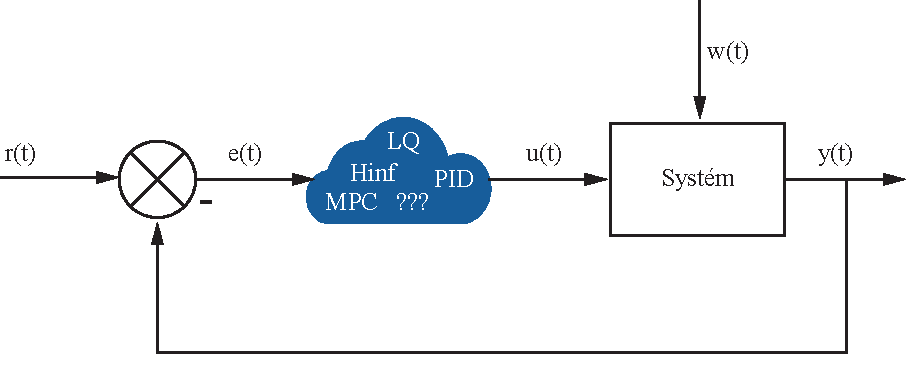
\includegraphics[width=80mm]{loop_Whatevs}\\
\end{figure}
\end{onlyenv}



\begin{onlyenv}<3->
\begin{figure}
\centering
  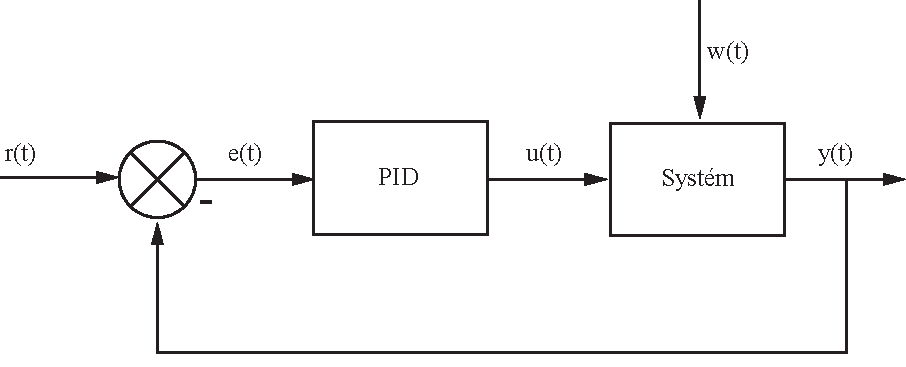
\includegraphics[width=80mm]{loop_PID}\\
\end{figure}
\end{onlyenv}
\end{frame}


\begin{frame}[t]{Opakovanie: PID}
  \begin{itemize}
    \item<1-> \textbf{Súčasnosť} = proporcionálna zložka: okamžitá odchýlka $e(t)$, ale majme možnosť na ladenie, tak $K_Pe(t)$.
    \item<2-> \textbf{Minulosť} = integračná zložka: celková odchýlka $e(t)$ v minulosti, ale majme možnosť na ladenie, tak $K_I\int_0^te(t)\mathrm{d}t$.
    \item<3-> \textbf{Budúcnosť} = derivačná zložka: projektovaná odchýlka $e(t)$ do budúcnosti, ale majme možnosť na ladenie, tak $K_D\frac{\mathrm{d}e(t)}{\mathrm{d}t}$.
  \end{itemize}

\begin{onlyenv}<1>
\begin{figure}
\centering
  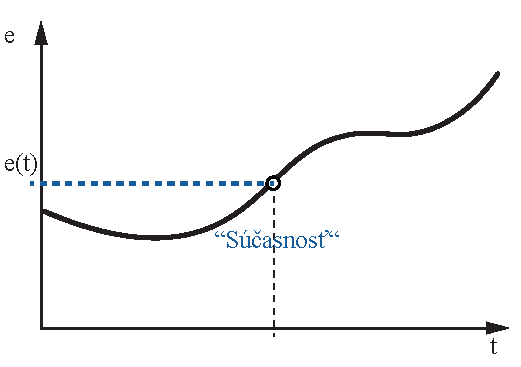
\includegraphics[width=50mm]{PID_P}\\
\end{figure}
\end{onlyenv}

\begin{onlyenv}<2>
\begin{figure}
\centering
  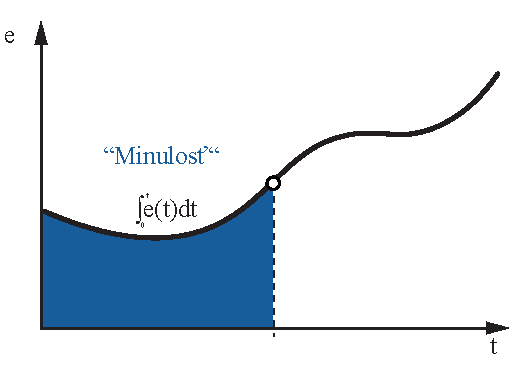
\includegraphics[width=50mm]{PID_I}\\
\end{figure}
\end{onlyenv}

\begin{onlyenv}<3>
\begin{figure}
\centering
  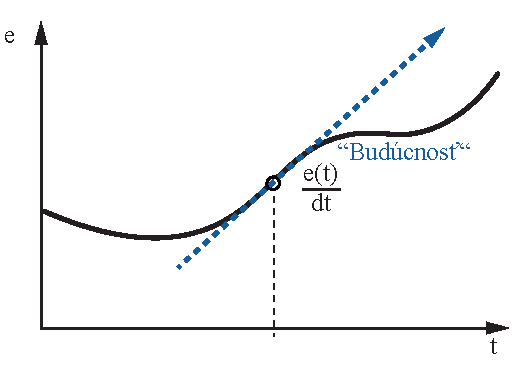
\includegraphics[width=50mm]{PID_D}\\
\end{figure}
\end{onlyenv}


\begin{onlyenv}<4->
tzv. paralelná (ideálna) forma
\begin{align}
u(t)= K_Pe(t)+K_I\int_0^te(t)\mathrm{d}t+K_D\frac{\mathrm{d}e(t)}{\mathrm{d}t}
\end{align}
\end{onlyenv}

\begin{onlyenv}<5>
alebo tzv. štandardná forma\footnote{V PX4 môžete prepínať pre rate controller \cite{PX4:PIDTuning}} (máme intuitívnejšie časové konštanty, ale zosilnenie je nezávislé\footnote{pozor, neintutívne...})
\begin{align}
u(t)= K_P\left(e(t)+\frac{1}{T_I}\int_0^te(t)\mathrm{d}t+T_D\frac{\mathrm{d}e(t)}{\mathrm{d}t}\right)
\end{align}
\end{onlyenv}
\end{frame}




\begin{frame}[t]{Opakovanie: Vzorkovanie, tvarovanie}
  \begin{itemize}
  \item<1-> Výpočtová realizácia neumožní počítať spojito, preto
    \begin{itemize}
      \item Vzorkujeme na strane výstupov --- ADC + slučka v hard real-time pomocou časovačov
      \item Tvarujeme na strane vstupov --- zero order hold (ZOH) len znamená podržíme hodnotu počas vzorky
    \end{itemize}
  \item<2-> Vzorkovanie mení spojitý čas na $t=kT_s$. Perióda je voliteľná, ale
    \begin{itemize}
      \item musí zachytiť dominantnú dynamiku riadeného deja,
      \item a výpočtová realizácia musí stíhať.
  \end{itemize}
\end{itemize}
\begin{figure}
\centering
  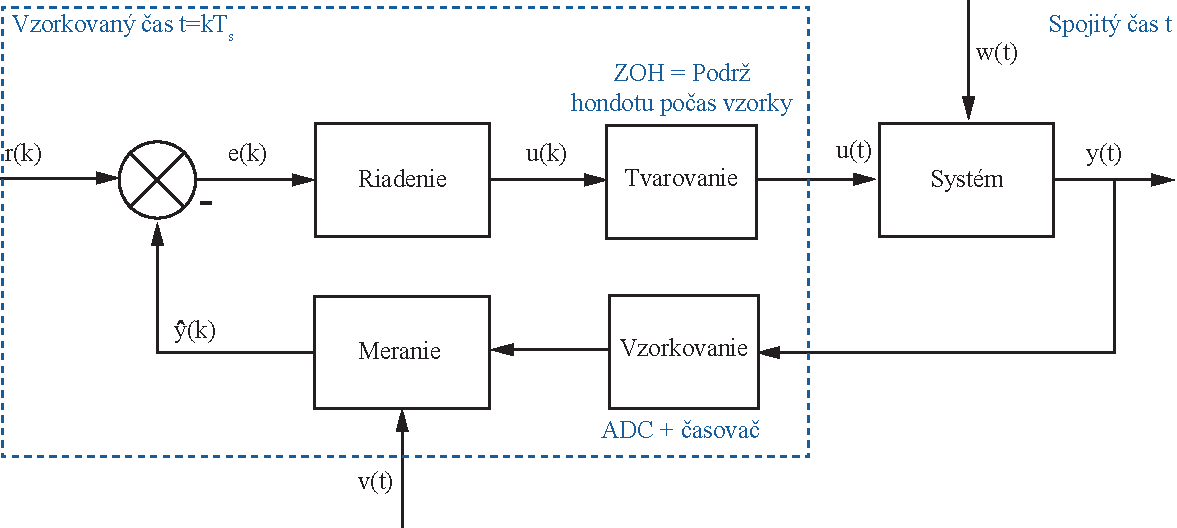
\includegraphics[width=0.9\textwidth]{loop_Sampling}\\
\end{figure}
\end{frame}


\begin{frame}[t]{Opakovanie: Číslicové PID}
  \begin{itemize}
    \item<1-> Systém, resp. proces zostáva spojitý\footnote{Samozrejme máme aj nespojité procesy a systémy}
    \item<2-> Koncepty ako integrácia, derivácia musíme numericky aproximovať, t.j. ak $T_s$ je vzorkovací čas, naše PID bude
        \begin{align}
        u(k)= K_Pe(k)+K_I\underbrace{\sum_0^te(k)T_s}_{\mathrm{``obdlzniky''}}+K_D\underbrace{\frac{e(k)-e(k-1)}{T_s}}_{\mathrm{``vstupanie''}}
        \end{align}
    \item<3->  alebo v prakticky vhodnejšej tzv. inkrementálnej forme pre MCU (bez dôkazu, viď. \cite{W:PID})
        {\scriptsize
        \begin{align}
        u(k)=u(k-1)+\left(K_P+K_IT_s+\frac{K_D}{T_s}\right)e(k)+\left(-K_P -2\frac{K_D}{T_s}\right)e(k-1)+\frac{K_D}{T_s}e(k-2)
         \end{align}
         }
\end{itemize}
\end{frame}




%\begin{frame}{Opakovanie: Riadená sústava}
%  \begin{itemize}
%    \item<1-> blah
%    \item<2-> blah blah
%  \end{itemize}

%%\begin{onlyenv}<1>
%\begin{figure}
%\centering
%  \includegraphics[width=\textwidth]{loop_full}\\
%\end{figure}
%%\end{onlyenv}
%\end{frame}
% 

\begin{frame}{Riadená sústava}
\begin{figure}
\centering
  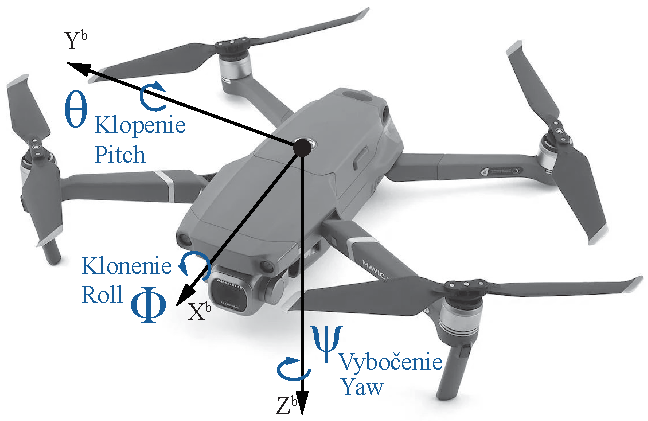
\includegraphics[width=\textwidth]{rollpitch}\\
\end{figure}
\end{frame}


\begin{frame}[t]{Rýchlosť zmeny uhlov / orientácie}
\begin{itemize}
  \item<1-> Tvárme sa, že poznáme žiadanú uhlovú rýchlosť orientácie $r_{\dot{\Theta}}$, $r_{\dot{\Phi}}$ a $r_{\dot{\Psi}}$ a pre jednoduchosť sústredme len na rýchlosť zmeny klopenia ($\dot{\Theta}$).
  \item<2-> Sme na najnižšej úrovni, t.j. riadenie uhlovej rýchlosti \angl{rate controller} --- je to zároveň aj najdôležitejšia slučka, a máme 3 nezávislých slučiek \citep{AP:PID,PX4:PIDTuning}
  \item<3->  Je to aj najrýchlejšia slučka (cca. $f_s$=400--1000 Hz \citep{AP:PID,PX4:PIDTuning})
  \end{itemize}

  \begin{onlyenv}<1>
  \begin{figure}
\centering
  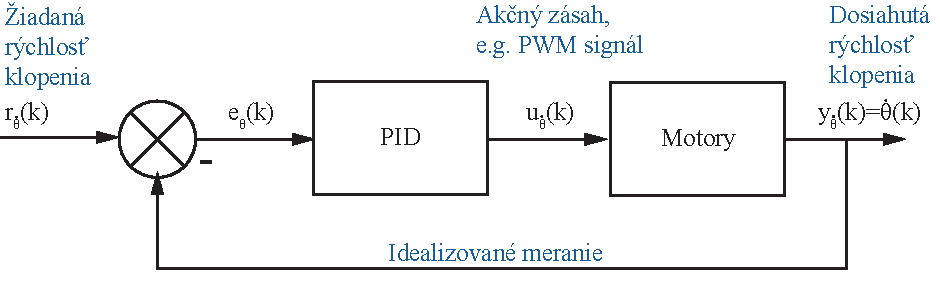
\includegraphics[width=\textwidth]{ATT_Rate}\\
\end{figure}
\end{onlyenv}

  \begin{onlyenv}<2-3>
  \begin{figure}
\centering
  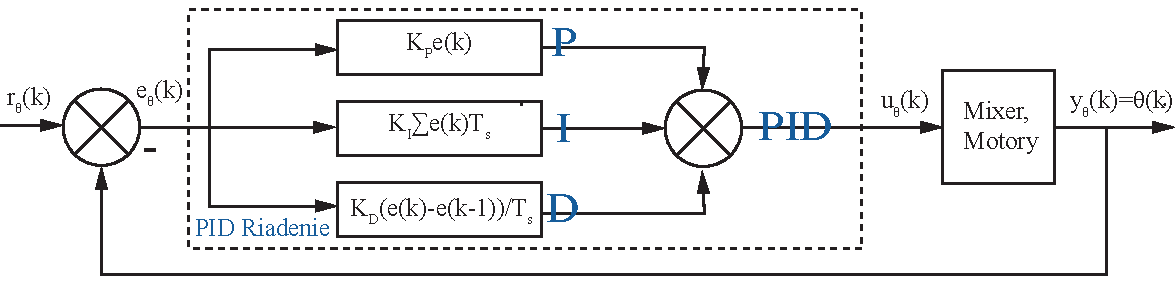
\includegraphics[width=\textwidth]{ATT_Rate2}\\
\end{figure}
\end{onlyenv}

  \end{frame}

\begin{frame}[t]{Ohraničenie vstupov}
  \begin{itemize}
    \item<1-> Akčné zásahy majú svoje ohraničenia (\angl{constraints})
    \item<2-> Ako donútime ich dodržanie? Saturáciou (orezávaním) hodnôt, ktoré skutočne vypočíta PID.
    \item<3-> Saturácia vnáša nelinearitu, vplýva na výkon riadenia aj stabilitu.
    \item<4-> Aj iné veličiny môžeme saturovať, napr. žiadané hodnoty. Ako by sme ohraničili výstup?
  \end{itemize}

    \begin{onlyenv}<2->
  \begin{figure}
\centering
  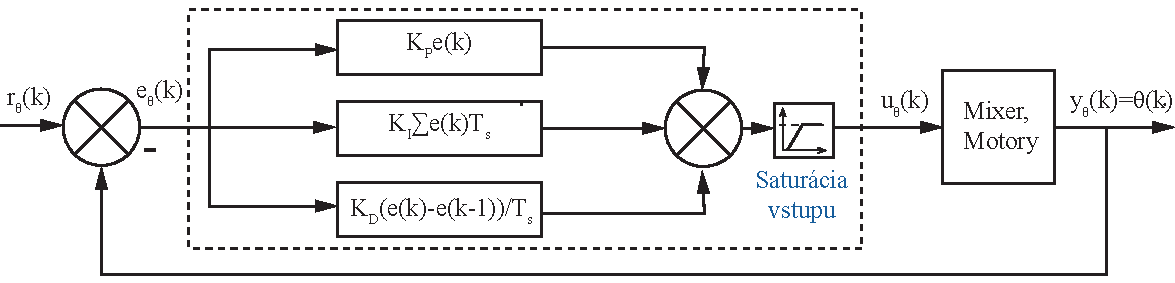
\includegraphics[width=\textwidth]{ATT_Rate3}\\
\end{figure}
\end{onlyenv}
\end{frame}


\begin{frame}[t]{Nahromadenie integračnej zložky}
  \begin{itemize}
    \item<1-> Integračná zložka ráta odchýlku v minulosti, preto ak akčné členy sú už na hraniciach možností - začína sa nahromaďovať \angl{windup}.
    %alebo sa to zbtočne nahromadí/začína sa zbytočne nahromaďovať (nemôže sa yačínať robiť sloveso v dokonavom vide...)
    \item<2-> Akonáhle sa vrátia akčné zásahy pod ohraničenia, nahromadená I zložka stále bude tlačiť systém na hranice možností, musí sa to chvíľu ``uvoľňovať'' \angl{unwind} a tým pádom prestrelíme \angl{overshoot} žiadané hodnoty
    \item<3-> To je saturácia integračnej zložky \angl{integral windup}.
    \item<4-> Môžeme používať rôzne triky, napr. ohraničiť veľkosť integračnej zložky, resp. vypnúť zložku pri určitých podmienkach.
  \end{itemize}
      \begin{onlyenv}<1-4>
  \begin{figure}
\centering
  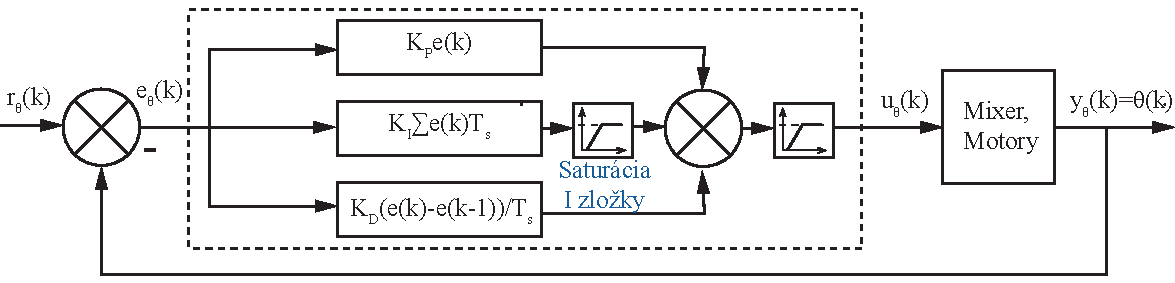
\includegraphics[width=\textwidth]{ATT_Rate4}\\
\end{figure}
\end{onlyenv}

      \begin{onlyenv}<5>
        \begin{itemize}
  \item<1-> ArduPilot - Ak akčný člen je akurát saturovaný, podrž hodnotu I zložky. Nižšie to môže ísť, vyššie nie \citep{AP:PID}.
  \item<2-> ArduPilot - Keďže máme kaskádnu konfiguráciu PID slučiek, saturačný znak postupuje cez hierarchiu nižšie a nižšie aby zastavil nahromadenie I zložky \citep{AP:PID}.
            \end{itemize}
      \end{onlyenv}

\end{frame}



\begin{frame}[t]{Šum a kopnutie derivačnej zložky}
  \begin{itemize}
    \item<1-2> Šum zo snímačov môže propagovať cez výpočet odchýlky riadenia do derivačnej zložky Vysokofrekvenčné zložky potom navýšia D zložku (čo je derivácia impulzu?)
    \item<2> Riešenie: Odchýlku riadenia pustíme cez dolnopriepustný \angl{low-pass} filter (LPF) --- Aj ArduCopter (20 Hz LPF) aj PX4 Autopilot používa \citep{AP:PID,PX4:PID}
    \item<3-> Náhle zmeny spôsobia ``kopnutie'' riadenia \angl{derivative kick}. (čo je derivácia impulzu?)
    \item<4-> Môžeme celkovo obísť zmenu žiadanej hodnoty a tým odchýlky  $e_\Theta(k)$ tak, že derivujeme výstup $y_\Theta(k)$\footnote{Riešenie v PX4, ArduCopter používa input shaping.}
  \end{itemize}
      \begin{onlyenv}<1-2>
  \begin{figure}
\centering
  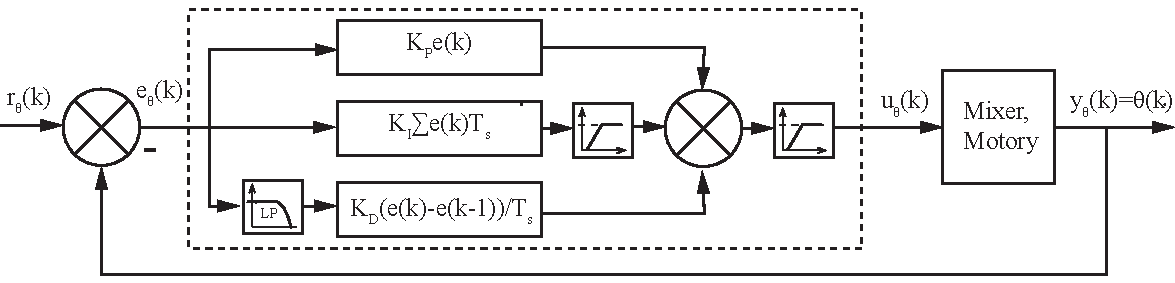
\includegraphics[width=\textwidth]{ATT_Rate5}\\
\end{figure}
\end{onlyenv}

\begin{onlyenv}<3->
  \begin{figure}
\centering
  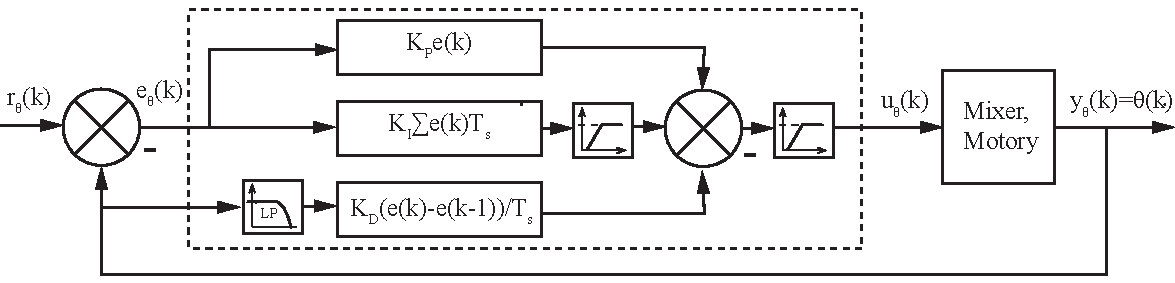
\includegraphics[width=\textwidth]{ATT_Rate6}\\
\end{figure}
\end{onlyenv}


\end{frame}

\begin{frame}
  \begin{figure}
\centering
  \includegraphics[width=100mm]{PX4_Rate}\\
\end{figure}

\end{frame}
%\input{_02_PID_Attitude.tex}


\begin{frame}
DCM -> Direction Cosine Matrix (pre 3.2)
Transformation to inertial to body axes.
Quaternion 4 by 1
\end{frame}


\begin{frame}[t]{Orientácia}
\begin{itemize}
  \item<1-> riadenie orientácie, tj. uhly $\Omega={\Phi, \Theta, \Sigma}$ a uhlové rýchlosti $\dot\Omega$ v ''body frame``
  \item<2-> Pre RC dron by to aj stačilo s plynom $\tau$ \angl{throttle}\footnote{Síce rate-control je tiež možné \citep{Boland2015}!} \citep{Boland2015}
  \item<3-> Riadiť orientáciu \angl{attitude} len na základe zmeny uhl. rýchlosti \angl{rate} by bolo dosť neintuitívne, potrebujeme prepočítať $r_{\Theta} \rightarrow r_{\dot{\Theta}}$
\end{itemize}
\end{frame}


\begin{frame}[t]{Orientácia}
\begin{itemize}
  \item<1-> Tvárme sa, že poznáme žiadané orientácie (napr. RC), napr. klopenie $r_{\Theta}$ a chceme riadiť $y_{\Theta}$.  V skutočnosti riešené s kvaterniónmy aby sme obišli singularitu Eulerových uhlov pri odhade \citep{Erasmus2020}.
  \item<2-> Riadenie orientácie môže byť riešené ďalšou, nadradenou regulačnou slučkou - hovoríme o tzv. kaskádnom riadení \angl{nested, cascaded}.
  \end{itemize}


    \begin{onlyenv}<1-2>
  \begin{figure}
\centering
  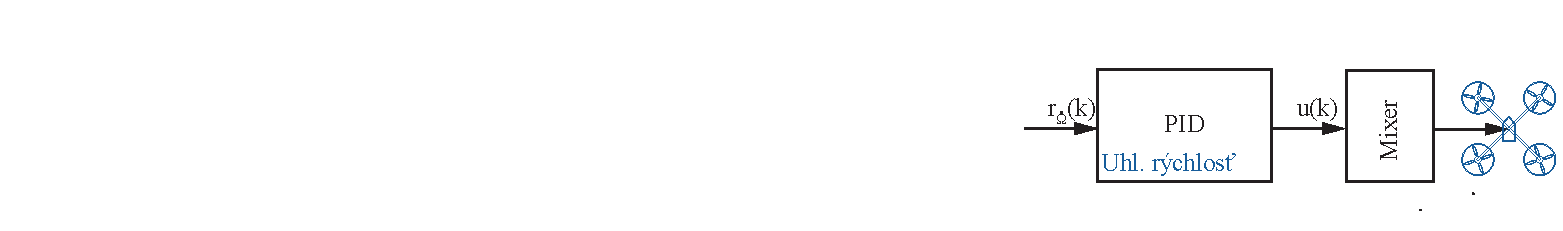
\includegraphics[width=\textwidth]{PID_HighLevel1a}\\
\end{figure}
\end{onlyenv}



    \begin{onlyenv}<3>
  \begin{figure}
\centering
  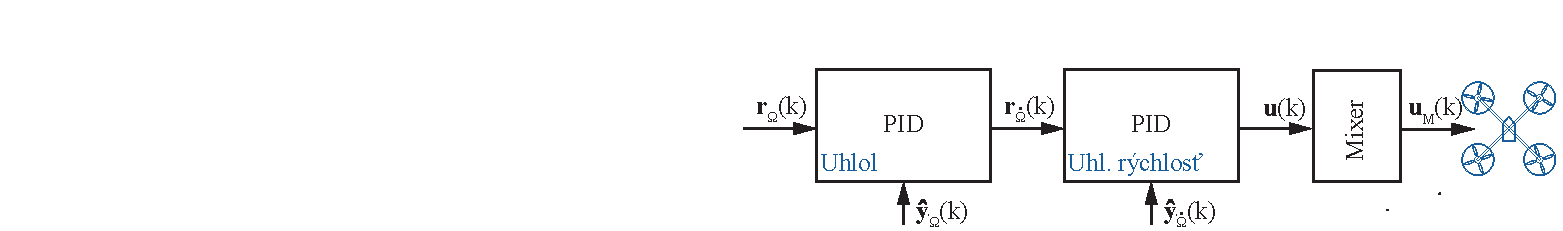
\includegraphics[width=\textwidth]{PID_HighLevel1b}\\
\end{figure}
\end{onlyenv}

  \end{frame}



\begin{frame}[t]{Orientácia 2}
\begin{itemize}
  \item<1-> Nadradené slučky sú pomalšie, vytvára to istý ``filter'', t.j. nemôžeme rýchlejšie ovládať rýchlosť ako polohu (cca. o rád, min polovicu pomalšie\footnote{ArduCopter 40 Hz vs 400 Hz, PX4 250 vs. 1000 Hz \citep{AP:PID,PX4:PID}}) \citep{AP:PID,PX4:PID}
  \item<2-> Pri PID skôr P\footnote{ArduCopter a PX4 Autopilot používa P regulátor \citep{PX4:PID,AP:PIDDOC}}, lebo reaguje príliš agresívne na šum.
  \item<3-> Do slučky dopracujeme doprednú väzbu \angl{feedforward} ktorá zrýchli odozvu regulácie. ``Whatever works'' - netreba mystifikovať.
  \end{itemize}



  \begin{onlyenv}<2>
  \begin{figure}
\centering
  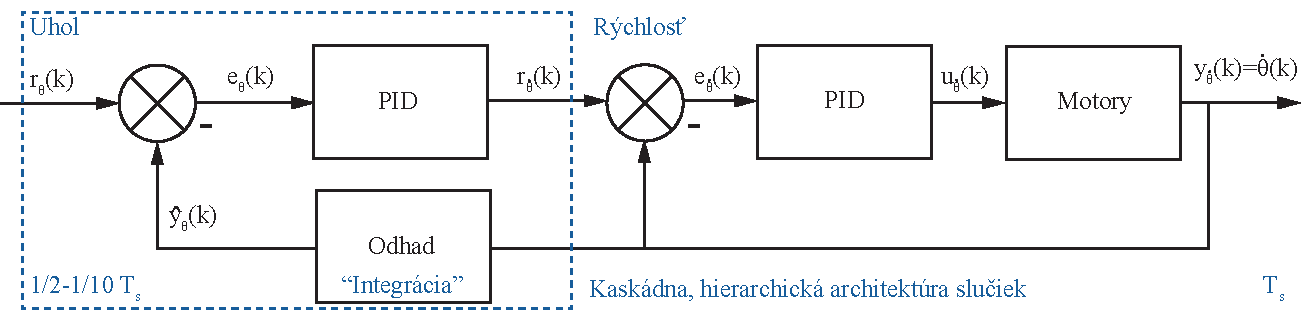
\includegraphics[width=\textwidth]{ATT_Angle}\\
\end{figure}
\end{onlyenv}

  \begin{onlyenv}<3->
\begin{figure}
\centering
  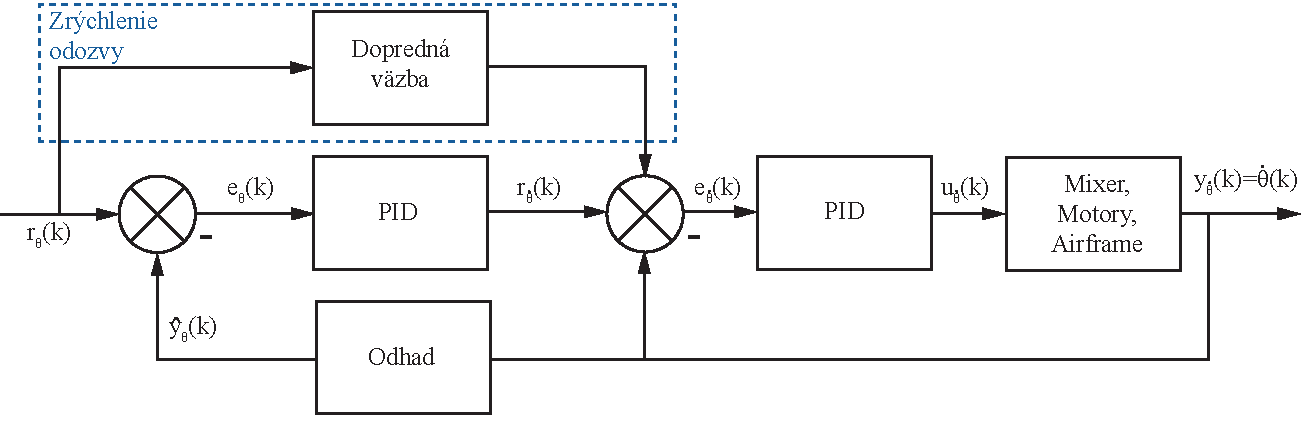
\includegraphics[width=\textwidth]{ATT_Angle2}\\
\end{figure}
\end{onlyenv}

  \end{frame}



  \begin{frame}[t]{Orientácia 3}
\begin{itemize}
  \item<1-> PX4 používa kvaternióny, ale je to iba P regulátor
  \item<2-> ArduCopter v podstate taktiež tam má P regulátor + FF
\end{itemize}

  \begin{onlyenv}<1->
  \begin{figure}
\centering
  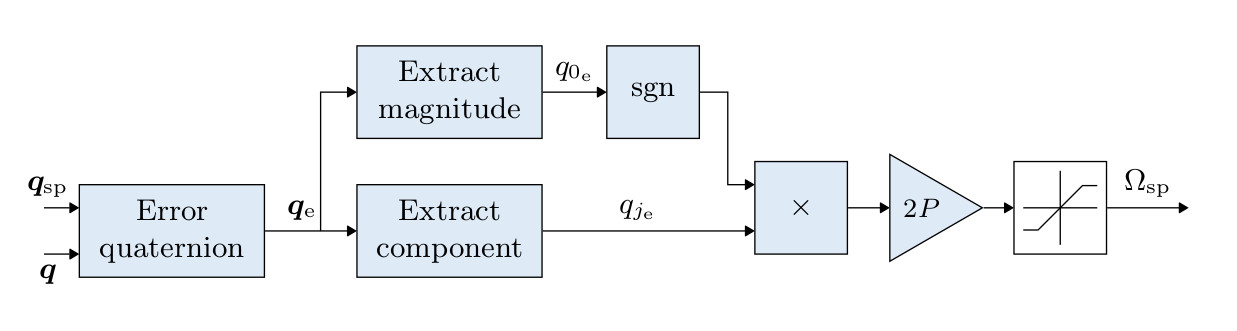
\includegraphics[width=100mm]{PX4_Angle}\\
\end{figure}
\end{onlyenv}


  \begin{onlyenv}<2->
  \begin{figure}
\centering
  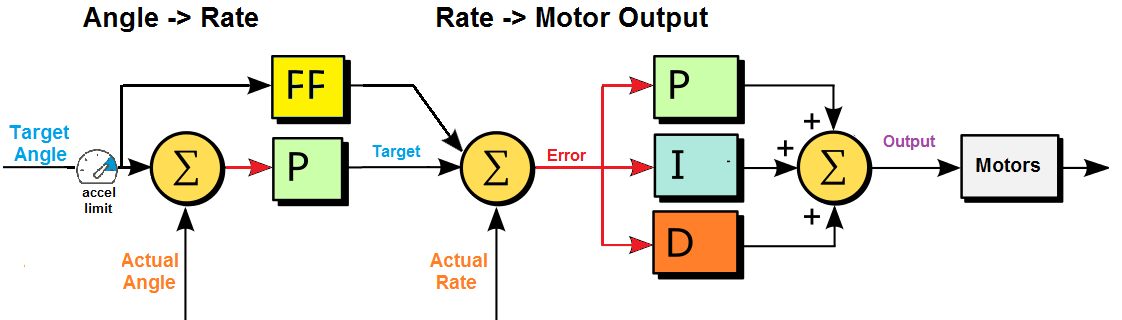
\includegraphics[width=80mm]{AP_Angle}\\
\end{figure}
\end{onlyenv}

  \end{frame}



  \begin{frame}[t]{Zmena súradníc}
\begin{itemize}
  \item<1-> aaaa
\end{itemize}

  \begin{onlyenv}<1->
  \begin{figure}
\centering
  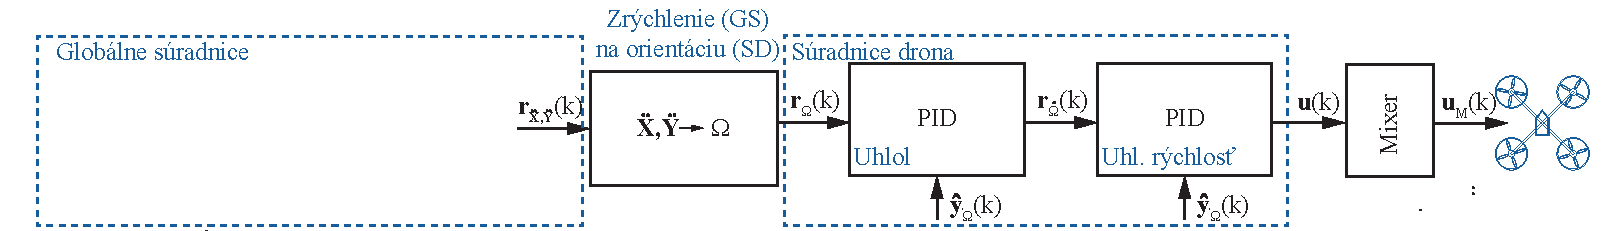
\includegraphics[width=\textwidth]{PID_HighLevel2}\\
\end{figure}
\end{onlyenv}

  \end{frame}



  \begin{frame}[t]{Rýchlosť}
\begin{itemize}
  \item<1-> aaaa
\end{itemize}

  \begin{onlyenv}<1->
  \begin{figure}
\centering
  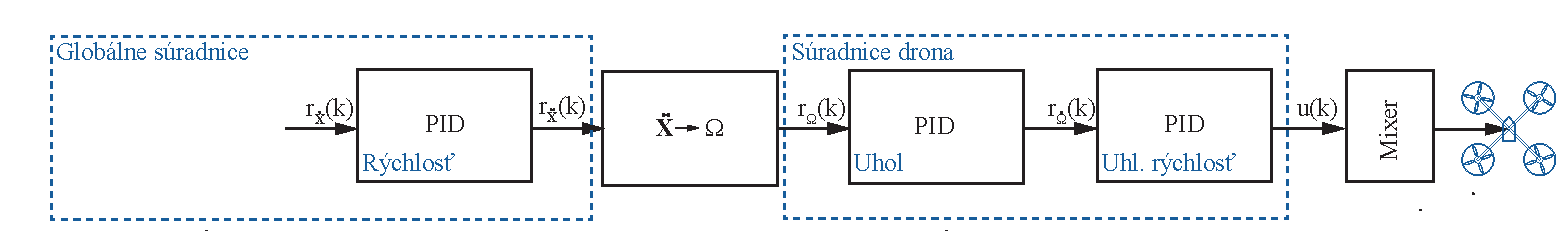
\includegraphics[width=\textwidth]{PID_HighLevel3}\\
\end{figure}
\end{onlyenv}


  \begin{onlyenv}<2->
  \begin{figure}
\centering
  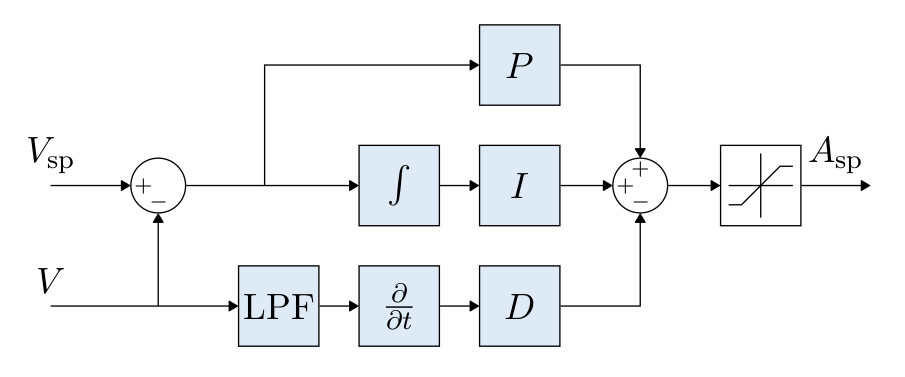
\includegraphics[width=70mm]{PX4_Velocity}\\
\end{figure}
\end{onlyenv}

  \end{frame}


 \begin{frame}[t]{Poloha}
\begin{itemize}
  \item<1-> aaaa
\end{itemize}

  \begin{onlyenv}<1->
  \begin{figure}
\centering
  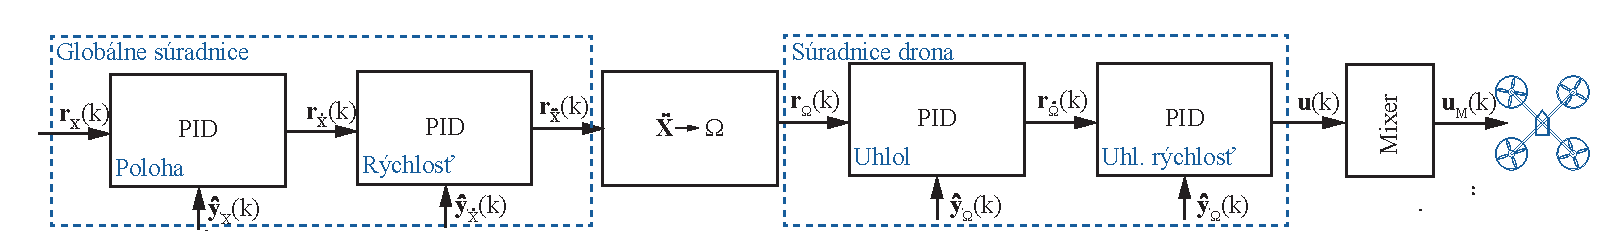
\includegraphics[width=\textwidth]{PID_HighLevel4}\\
\end{figure}
\end{onlyenv}


  \begin{onlyenv}<2->
  \begin{figure}
\centering
  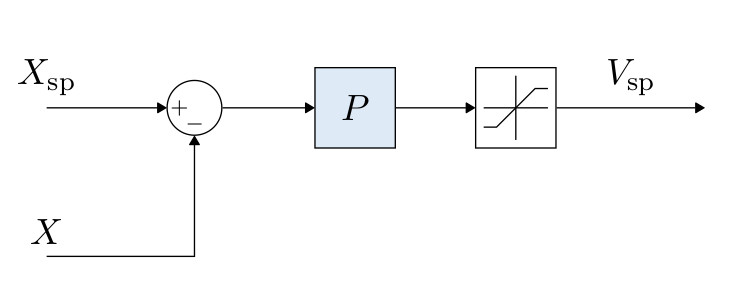
\includegraphics[width=50mm]{PX4_Position}\\
\end{figure}
\end{onlyenv}
  \end{frame}




\begin{frame}[t]{Tvarovanie žiadaných hodnôt}
  \begin{itemize}
  \item<1-> Dron je stabilizovaný, pilot/ROS náhle chce $r_{\Phi}=$+30$^\circ$ klonenie. Čo sa stane s riadením?
  \item<2->  Žiadaná hodnota je skokový signál. Derivácia skoku je... D zložka a tým aj vstup do akčných členov vystrelí!
  \item<3->  Potrebujeme tvarovať vstupy do regulácie \angl{input shaping}, t.j. tvarovať žiadané hodnoty:
        \begin{itemize}
  \item Pomalšie vzorkovanie na rýchlejšie (interpolácia) \footnote{ArduCopter 50 Hz $\rightarrow$ 400 Hz \citep{AP:PID}}
  \item Vyhladenie filtráciou, saturácie
  \item<4-> Ak hovoríme o manuálnom pilotovaní, tvarovanie určuje aký ``pocit'' je riadiť stroj
  \end{itemize}
  \end{itemize}

        \begin{onlyenv}<2>
  \begin{figure}
\centering
  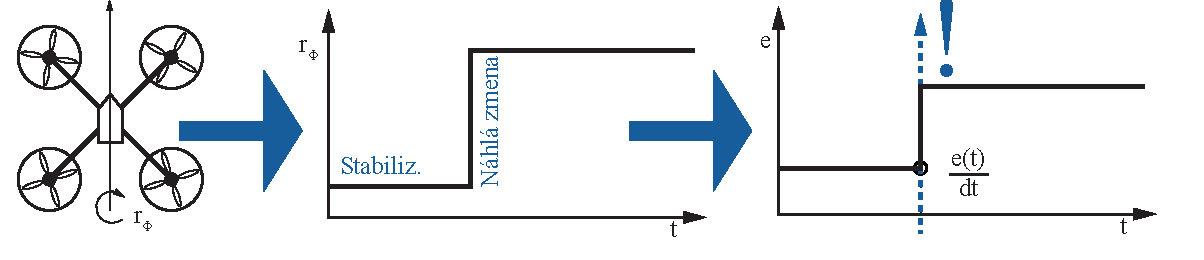
\includegraphics[width=\textwidth]{InputShaping_1}\\
\end{figure}
\end{onlyenv}


        \begin{onlyenv}<3->
  \begin{figure}
\centering
  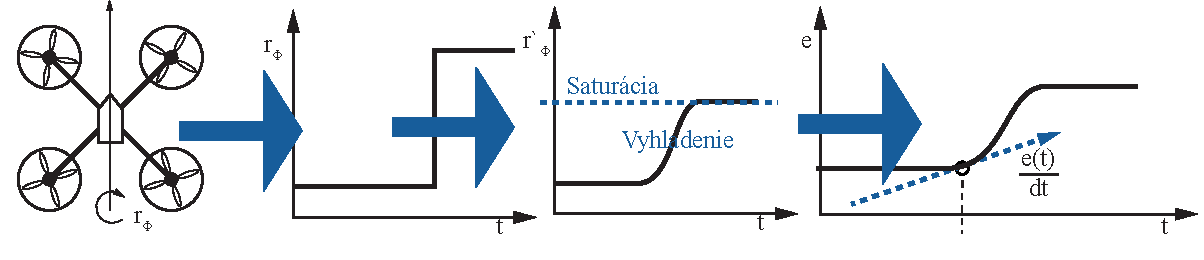
\includegraphics[width=\textwidth]{InputShaping_2}\\
\end{figure}
\end{onlyenv}







\end{frame}

\begin{frame}[t]{Inicializácia riadenia}
\begin{itemize}
  \item<1-> Ako naštartujeme riadenie? Aká je odchýlka $e(0)$ pri štarte?
  \item<2-> Kritické pri zmene letových módov \citep{AP:PID,Bresciani2020}
  \item<3-> Pre ArduCopter \cite{AP:PID}
    \begin{itemize}
    \item Nadradené riadenie poloha vs. rýchlosť (P) --- tak aby vstup bol konštantný
    \item Rýchlosť (PID) --- $e(0)=0$, I zložka s konštantným vstupom, zrátať D pri nastavení žiadanej hodnoty
\end{itemize}

\end{itemize}
\end{frame}






\begin{frame}{Je perfektné sledovanie trasy možné?}
\begin{itemize}
\item<1-> Majme trasu WP1 do WP2, všetko je v poriadku.
\item<2-> Pridajme WP3 a rozmýšľajme čo sa deje pri WP2. Je možné preletieť nad WP2?
\item<3-> Buď musíme úplne sa zastaviť alebo nemôžeme priamo preletieť --- ináč by sme potrebovali nekonečne veľké zrýchlenia
\end{itemize}

\begin{onlyenv}<1>
  \begin{figure}
\centering
  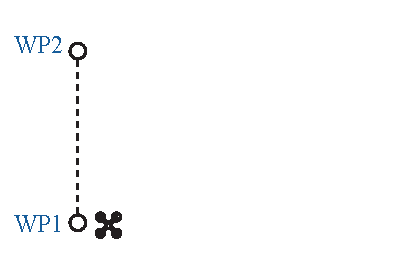
\includegraphics[width=60mm]{PositionControl}\\
\end{figure}
\end{onlyenv}

\begin{onlyenv}<2>
  \begin{figure}
\centering
  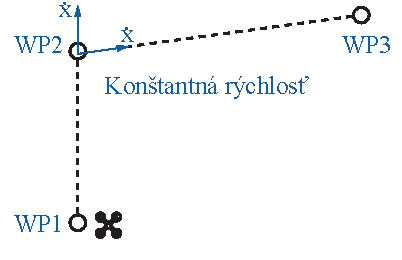
\includegraphics[width=60mm]{PositionControl2}\\
\end{figure}
\end{onlyenv}

\begin{onlyenv}<3>
  \begin{figure}
\centering
  \includegraphics[width=60mm]{PositionControl3}\\
\end{figure}
\end{onlyenv}


\end{frame}


\begin{frame}[t]{Automatické nastavenie parametrov}
\begin{itemize}
  \item ArduPilot (ArduCopter) --- Napodobňuje heuristiku \citep{AP:LogSeminar}
  \begin{itemize}
  \item Zvyšuje D parameter pomaly
  \item Akonáhle deteguje osciláciu, zníži D parameter
  \item Opakuje pre iné zložky/slučky
\end{itemize}
\item Intuitívne ale konzervatívne
\end{itemize}

\end{frame}



\begin{frame}
Notes: \cite{AP:PID}

User (ROS) $\rightarrow$ Shaping $\rightarrow$ PID $\rightarrow$ Actuators
Yaw je prioritizovanych nad Pitch Roll, lebo to drzi dron v lufte \citep{Erasmus2020}
50 Hz -> 400 Hz
Min 24 tazsie uchopytelne koncepty pre prezentaciu, dava menej konkretnosti
Velocity prioritizuje vertikalnu rychlost   \citep{Erasmus2020}
\end{frame}



\thankyouslide{gergely.takacs@stuba.sk}{SK}
\referencesslidebiber{SK}

%\backupbegin
%\input{...
%\backupend


\end{document}
